\documentclass[12pt]{article}
\usepackage{graphicx}
\usepackage{caption}
\usepackage{float}
\usepackage[a4paper,margin=1in,footskip=0.25in]{geometry}
\usepackage{pdfpages}
\usepackage{setspace}
\doublespace
% \usepackage[english]{babel}
% \usepackage[style=ieee,backend=biber]{biblatex}
% \addbibresource{lab.bib}
\usepackage{hyperref}
\hypersetup{
    colorlinks,
    citecolor=black,
    filecolor=black,
    linkcolor=black,
    urlcolor=black
}

\begin{document}

\title{Polyopticon SDS}
\author{Jon Bakies \and Mitchell Dunn} 

\maketitle
\newpage

\tableofcontents
\newpage

\section{Summary Of Proposal}
\paragraph{}
Polyopticon is a portable presentation tool that consists of a projector, camera, Raspberry Pi, and an infrared(IR) LED drawing tool.
The camera, pointed at the projected surface, will capture the user's pen strokes with image recogintion of the IR LED.
Originally the Raspberry Pi was intended to project and handle all of the image processing, but after testing it was determined that the Raspberry Pi could not handle such a demanding task.
Instead of performing the image recognition on the Raspberry Pi, the Pi will stream the video to the user's computer to be processed.

\section{Design}
\subsection{Dataflow}
\begin{figure}[ht!]
\centering
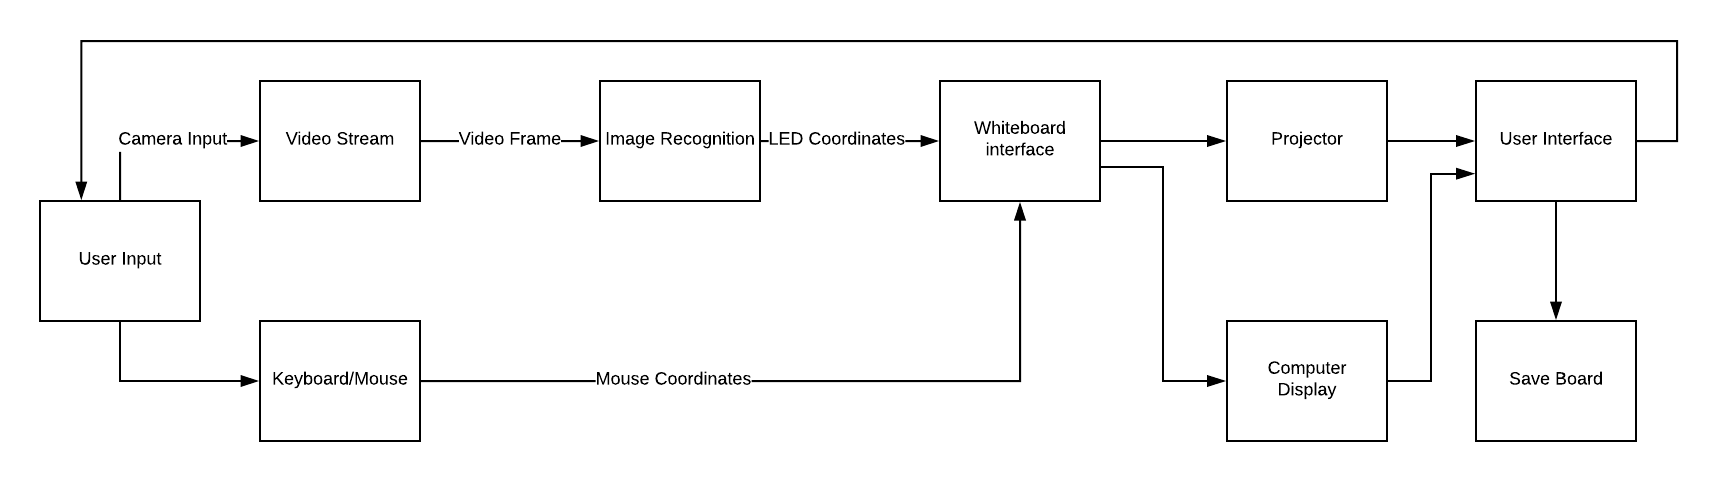
\includegraphics[width=\textwidth, height=\textheight, keepaspectratio]{Dataflow.png}
\end{figure}
\paragraph{}
The user can input data from the projected user interface via the IR LED and the camera, or from their personal computer where they can directly interact with the whiteboard interface.
The video from the camera is streamed to the user's computer and passed through openCV frame by frame to search for the LED.  
Once the LED is found, the coordinates are sent to the whiteboard interface to display pen strokes.
The whiteboard interface is projected and displayed on the user's computer, and makes up the user interface.
\subsection{Image Recognition}
\begin{figure}[H]
\centering
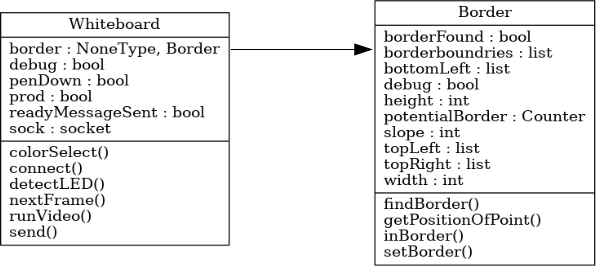
\includegraphics[scale=.5]{classdiagram.png}
\end{figure}
\paragraph{}
The Image Recognition part of Polyopticon is written in python and consists of two classes.
The Whiteboard class locates the LED in an image using openCV and sends the coordinates to the whiteboard interface through a socket.
The Border class stores information about the border of the drawable space, and conatins methods to determine if coordinates are within the border.


% \newpage \section{References} \printbibliography[heading=none]
\end{document}
